\section{\textsc{Spiegelei auf italienisch}}

\subsection*{Zutaten für 2 Portionen:}

\begin{tabular}{p{7.5cm} p{7.5cm}}
	& \\
	6 Eier & Mozzarella \\
	Öl zum Braten & Gewürze nach Geschmack
\end{tabular}

\subsection*{Serviervorschlag:}

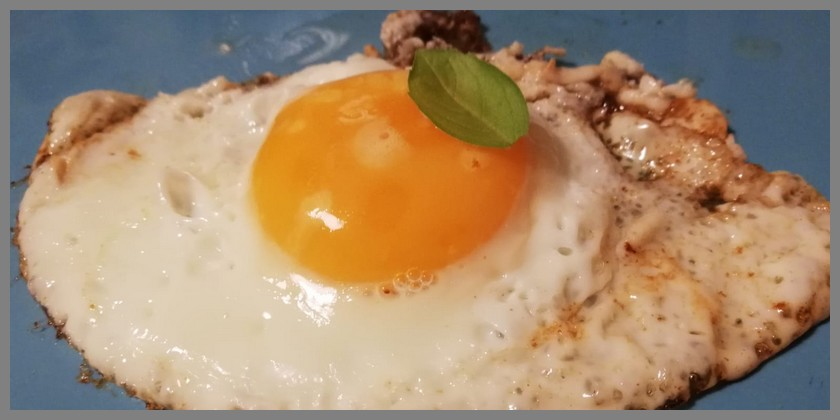
\includegraphics[width=\textwidth]{img/spiegelei.jpg} \cite{itaspiegelei}

\subsection*{So geht's:}

\begin{tabular}{p{15cm}}
	\\
  Öl in der Pfanne erhitzen.\\
  Tomate in dünne Scheiben schneiden und in der Pfanne andünsten.\\
  Nun die Eier in die Pfanne schlagen.\\
  Sobald es anfängt zu stocken, den Mozzarella gleichmäßig darauf verteilen.\\
  Würzen und fertig.
\end{tabular}
